\documentclass[10pt,a4paper]{article}
\usepackage[latin1]{inputenc}
\usepackage{amsmath}
\usepackage{amsfonts}
\usepackage{amssymb}
\usepackage{graphicx}

\author{Paul Wieland}
\title{INF3490 Mandatory Assignment 1}
\date{Deadline: September 21, 2018}
\begin{document}
	\maketitle
	\tableofcontents
	\newpage
%%%%%%%%%%%%%%%%%%%%%%%%%%%%%%%%%%%%%%%%%%%%%%%%%%%%%%%%%%%%%%%%%%%%%%%%%%%%%%%	
% General
%%%%%%%%%%%%%%%%%%%%%%%%%%%%%%%%%%%%%%%%%%%%%%%%%%%%%%%%%%%%%%%%%%%%%%%%%%%%%%%		
	\section{General}
	This assignment consists of four other files. The european\_cities.py, exhaustive\_search.py,  hill\_climbing.py, genetic\_algorithm.py and common.py. 
	So for each algorithm is one file given that can be executed. How to use them will be explained later.\\
	The common.py file is not meant to be executed.There are just some functions implemented that are used in several other files. For example the function \textit{calculate\_fitness(cities,data)} (line 14,common.py) calculates the total length of a specific route. How to use this functions is explained in the comments. So in fact this file should just avoid code redundancy.
	\\
	\\
	\textbf{All these functions have been successfully tested on a Ubuntu Linux 18.04 machine executed with python3.}
	\\
	\\
	Used libraries (to be sure that the files can be executed):
	\begin{itemize}
		\item timeit
		\item numpy
		\item random
		\item itertools
		\item sys
		\item matplotlib
	\end{itemize}
%%%%%%%%%%%%%%%%%%%%%%%%%%%%%%%%%%%%%%%%%%%%%%%%%%%%%%%%%%%%%%%%%%%%%%%%%%%%%%%	
% Exhausive Search
%%%%%%%%%%%%%%%%%%%%%%%%%%%%%%%%%%%%%%%%%%%%%%%%%%%%%%%%%%%%%%%%%%%%%%%%%%%%%%%		
	\section{Exhaustive Search}
	The following exhaustive search algorithm works very simple. It tries all possible combinations of how a set of cities can be visited. The actually implementation steps can be seen in the next subsection.
%%%%%%%%%%%%%%%%%%%%%%%%%%%%%%%%%%%%%%%%%%%%%%%%%%%%%%%%%%%%%%%%%%%%%%%%%%%%%%%	
% Exhausive Search,Code Overview
%%%%%%%%%%%%%%%%%%%%%%%%%%%%%%%%%%%%%%%%%%%%%%%%%%%%%%%%%%%%%%%%%%%%%%%%%%%%%%%	
	\subsection{Code Overview}	
	\begin{center}
		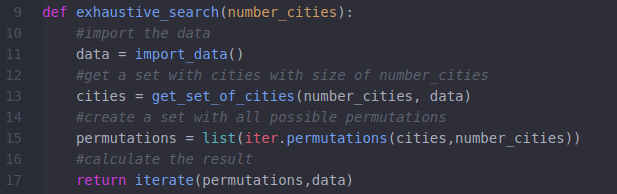
\includegraphics[width=1.0\linewidth]{pictures/exhaustiveSearch/code_exhaustive_search}
	\\
	Core function of exhaustive search	
	\\	
	\end{center}
	The function that can be seen in the graphic above is the core function because it handles the logic to determine the best solution. There are just three steps to explain in detail.\\
	In line 11 is the data imported from the csv file. In line 13 we can see that a subset of cities is created that has the size of the parameter number\_cities. In line 15 is the function permutations form the itertools used to determine all possible permutations. So the size of the variable permutations is exactly \textit{number\_cities!} (!: factorial).
	And last but not least is the function \textit{iterate()} called that iterates over all permutations to determine their fitness using \textit{calculate\_fitness(cities, data)}. The best solution will be returned.
%%%%%%%%%%%%%%%%%%%%%%%%%%%%%%%%%%%%%%%%%%%%%%%%%%%%%%%%%%%%%%%%%%%%%%%%%%%%%%%	
% Exhausive Search, Run the program
%%%%%%%%%%%%%%%%%%%%%%%%%%%%%%%%%%%%%%%%%%%%%%%%%%%%%%%%%%%%%%%%%%%%%%%%%%%%%%%	
	\subsection{Use the program}
	\subsubsection{Run the program}
	To run the program just execute the file: 
	\begin{center}
		\textit{python3 exhaustive\_search.py}
	\end{center}
	\subsubsection{Change parameter}
	
	\begin{center}
		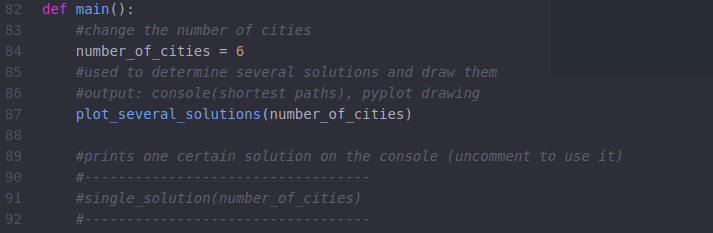
\includegraphics[width=1.0\linewidth]{pictures/exhaustiveSearch/use_the_program}
		\\
		Main function of exhaustive search
		\\
	\end{center}
	To change the number of cities that should be visited you can modify the parameter \textit{number\_of\_cities} to a number higher than zero.
	\\
	Per default is the function \textit{plot\_several\_solutions()} called. This function determines the best solution for different number of cities. All solutions are going to be printed to the console. This function creates also a graphical representation that shows the number of cities in terms to the run-time.
	\\
	\\
	It should look like this: 
	\begin{center}
		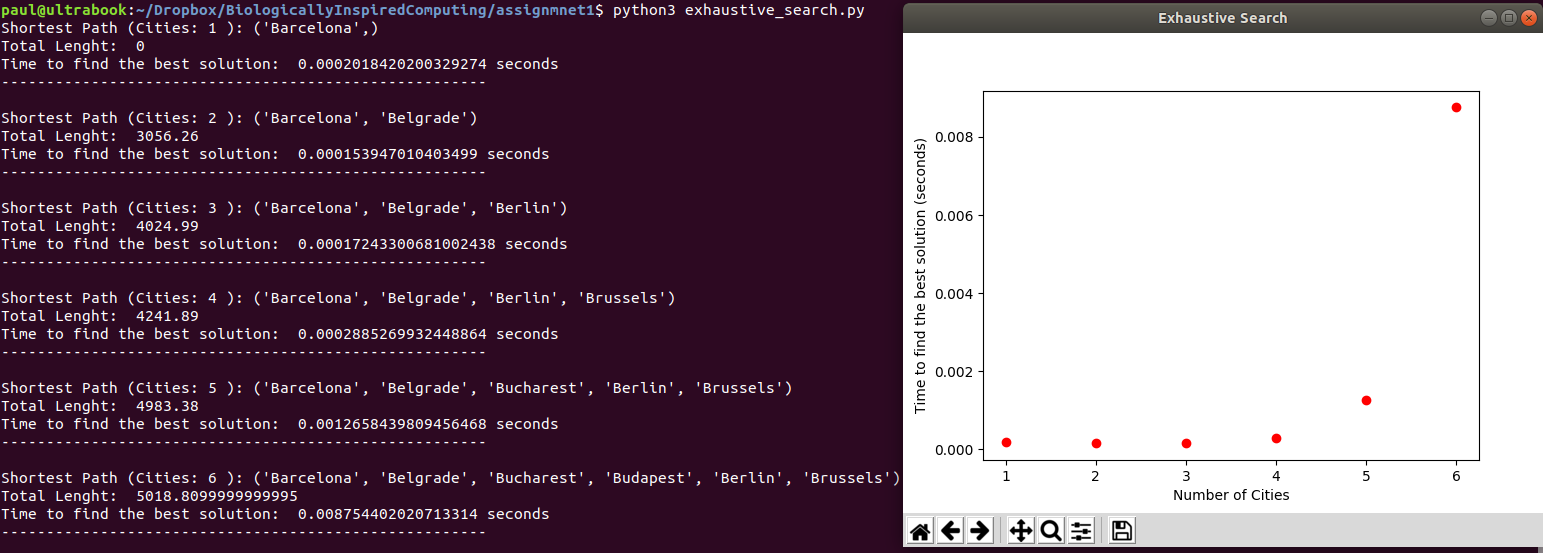
\includegraphics[width=1.0\linewidth]{pictures/exhaustiveSearch/plot_time_increasing}
		\\
		Output calling the function \textit{plot\_several\_solutions(6)}
		\\
	\end{center}
	But it is also possible to determine the solution for just one certain number of cities. For this you have to switch the comments in line 87 and line 91. So that the function \textit{single\_solution(number\_of\_cities)} is called. This function prints the solution to the console as you can see in 2.3.1.
%%%%%%%%%%%%%%%%%%%%%%%%%%%%%%%%%%%%%%%%%%%%%%%%%%%%%%%%%%%%%%%%%%%%%%%%%%%%%%%	
% Exhausive Search, Questions
%%%%%%%%%%%%%%%%%%%%%%%%%%%%%%%%%%%%%%%%%%%%%%%%%%%%%%%%%%%%%%%%%%%%%%%%%%%%%%%	
	\subsection{Questions}
	\subsubsection{Subset of 6 cities}
	\begin{center}
		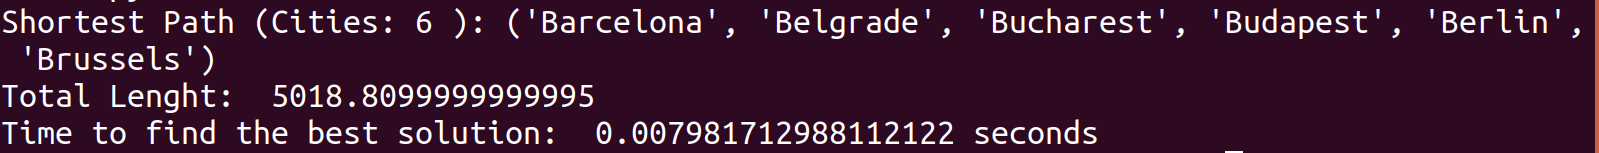
\includegraphics[width=1.0\linewidth]{pictures/exhaustiveSearch/cities6}
		Shortest path (subset of 6 cities)
	\end{center}
	
	\subsubsection{Incrementally add more cities}
	\begin{center}
		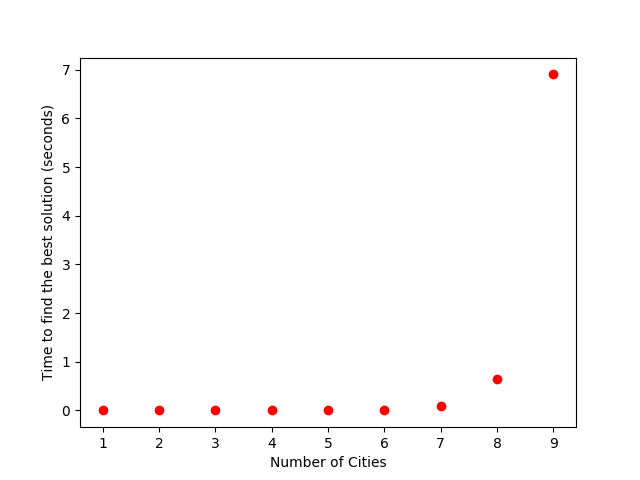
\includegraphics[width=0.8\linewidth]{pictures/exhaustiveSearch/exhaustive_search6}
	\end{center}
	The affect of adding more cities can bee seen very well in the graphic above. The run-time increases exponentially with the number of cities.
	
	\subsubsection{Subset of 10 cities}
	\begin{center}
		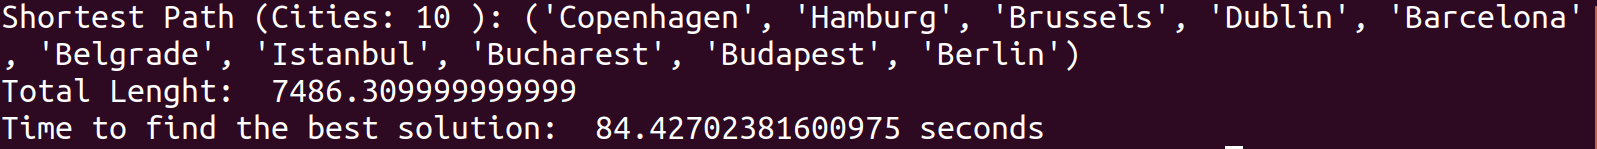
\includegraphics[width=1\linewidth]{pictures/exhaustiveSearch/cities10}
		\\
		Shortest Path (subset of 10 cities)
		\\
	\end{center}
	\begin{center}
		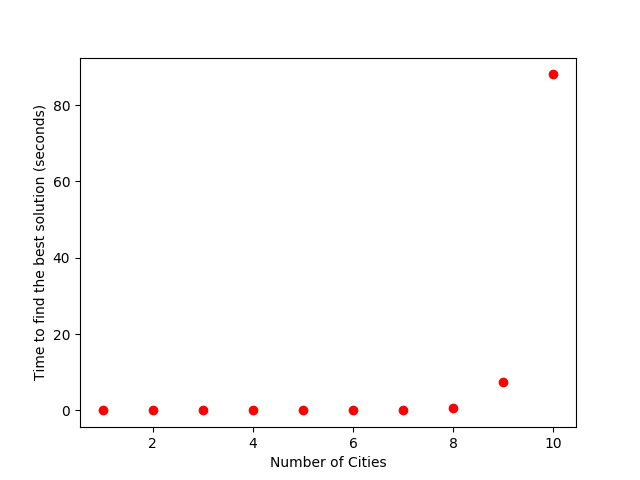
\includegraphics[width=0.8\linewidth]{pictures/exhaustiveSearch/exhaustive_search10}
		\\
		Graphical Representation
		\\
	\end{center}
	
	
	\subsubsection{Subset of 24 cities (expectation)}
	While a subset of 10 cities has 10! (3,628,800) possible solutions, a set with 24 cities has  620,448,401,733,239,439,360,000 possible solutions. So it is not possible to solve this in human live. It would take more than $4\times10^{11}$ years.
%%%%%%%%%%%%%%%%%%%%%%%%%%%%%%%%%%%%%%%%%%%%%%%%%%%%%%%%%%%%%%%%%%%%%%%%%%%%%%%	
% Hill Climbing
%%%%%%%%%%%%%%%%%%%%%%%%%%%%%%%%%%%%%%%%%%%%%%%%%%%%%%%%%%%%%%%%%%%%%%%%%%%%%%%	
	\section{Hill Climbing}
	The following hill-climbing implementation firstly creates a random order. To improve this initial solution, the algorithm swaps two cities an check if there is an improvement. A more detailed description can be seen in 3.1 and in the file \textit{hill\_climbing.py}.
%%%%%%%%%%%%%%%%%%%%%%%%%%%%%%%%%%%%%%%%%%%%%%%%%%%%%%%%%%%%%%%%%%%%%%%%%%%%%%%	
% Hill Climbing, Overview
%%%%%%%%%%%%%%%%%%%%%%%%%%%%%%%%%%%%%%%%%%%%%%%%%%%%%%%%%%%%%%%%%%%%%%%%%%%%%%%		 
	\subsection{Code Overview}
	\begin{center}
		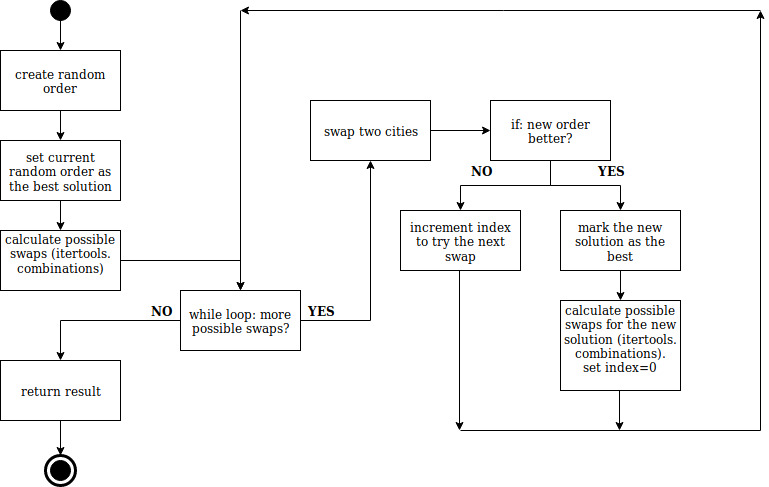
\includegraphics[width=1\linewidth]{pictures/hillClimbing/hill_climbing}
		\\
		Graphical representation of the function \textit{hill\_climbing(number\_of\_cities)}
		\\
	\end{center}
	The \textit{hill\_climbing(number\_of\_cities)} function is the heart of the hill-climber program. It just follows the steps you can see above in the flowchart. 
%%%%%%%%%%%%%%%%%%%%%%%%%%%%%%%%%%%%%%%%%%%%%%%%%%%%%%%%%%%%%%%%%%%%%%%%%%%%%%%	
% Hill Climbing, Use the program
%%%%%%%%%%%%%%%%%%%%%%%%%%%%%%%%%%%%%%%%%%%%%%%%%%%%%%%%%%%%%%%%%%%%%%%%%%%%%%%		
	\subsection{Use the program}
	\subsubsection{Run the program}
	To run the program just execute the file: 
	\begin{center}
		\textit{python3 hill\_climbing.py}
	\end{center}
	\subsubsection{Change parameter}
	\begin{center}
		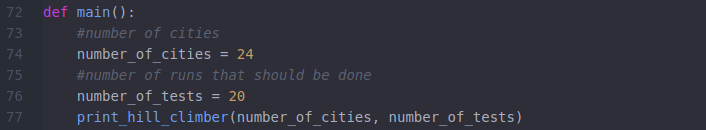
\includegraphics[width=1.0\linewidth]{pictures/hillClimbing/parameter}
		\\
		Main function of \textit{hill\_climbing.py}
		\\
	\end{center}

	\begin{tabular} {l l}
	number\_of\_cities: & Number of cities that should be visited \\
	number\_of\_tests : & Number of runs that should be made       \\
	\end{tabular}
	\\
	Per default is the function \textit{print\_hill\_climber(number\_of\_cities, number\_of\_tests)} called. The result of calling this function should look like 3.3.2 or 3.3.3.
%%%%%%%%%%%%%%%%%%%%%%%%%%%%%%%%%%%%%%%%%%%%%%%%%%%%%%%%%%%%%%%%%%%%%%%%%%%%%%%	
% Hill Climbing, Questions%%%%%%%%%%%%%%%%%%%%%%%%%%%%%%%%%%%%%%%%%%%%%%%%%%%%%%%%%%%%%%%%%%%%%%%%%%%%%%%	
% Hill Climbing
%%%%%%%%%%%%%%%%%%%%%%%%%%%%%%%%%%%%%%%%%%%%%%%%%%%%%%%%%%%%%%%%%%%%%%%%%%%%%%%	
%%%%%%%%%%%%%%%%%%%%%%%%%%%%%%%%%%%%%%%%%%%%%%%%%%%%%%%%%%%%%%%%%%%%%%%%%%%%%%%		
	\subsection{Questions}
	\subsubsection{Compare hill climbing to exhaustive search (10 cities)}
	\begin{center}
		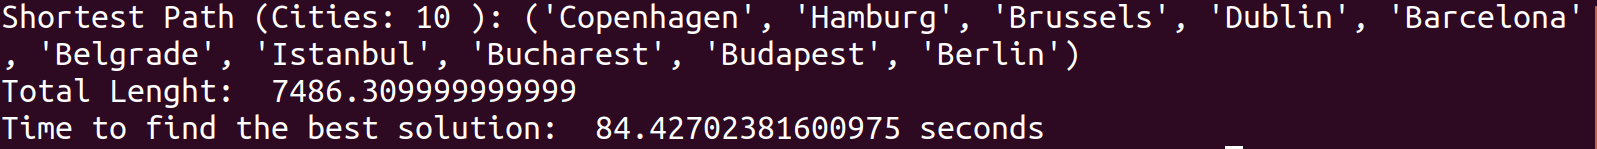
\includegraphics[width=1.0\linewidth]{pictures/exhaustiveSearch/cities10}
		\\
		Exhaustive Search, Shortest Path (subset of 10 cities)
		\\
	\end{center}

	\begin{center}
		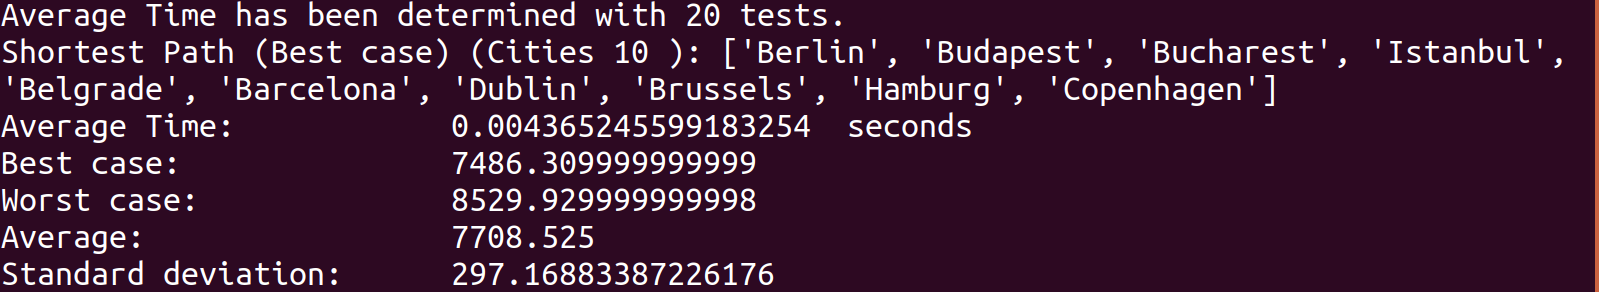
\includegraphics[width=1\linewidth]{pictures/hillClimbing/cities10}
		\\
		Hill Climbing Result, 10 Cities, 20 runs 
		\\	
	\end{center}
		As we can see, the hill climbing algorithm is much faster. For 10 cities:
		\\
		\begin{tabular}{ l l } 
		Exhaustive Search: & 82.4270 seconds \\
		Hill-Climbing (Average): & 00.0043 seconds  \\	
		\end{tabular}
	
	\subsubsection{Result 10 Cities, 20 runs}
	\begin{center}
		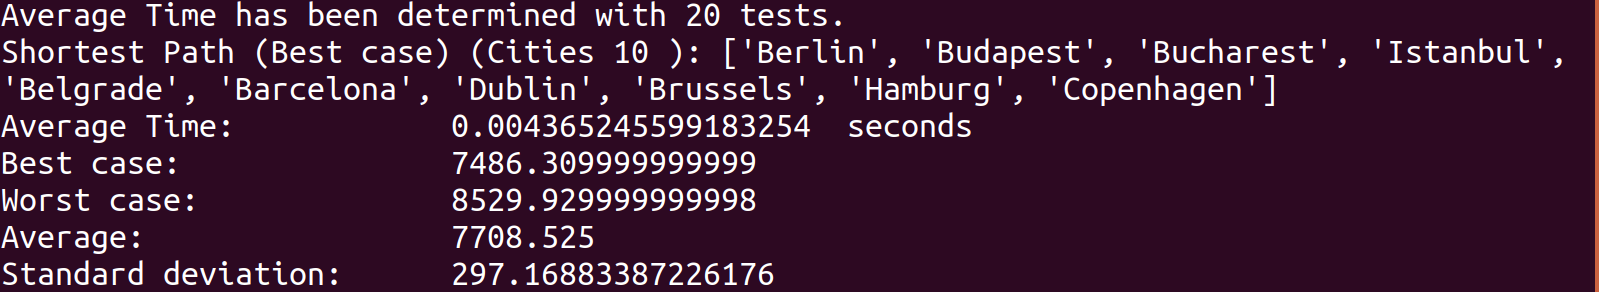
\includegraphics[width=1\linewidth]{pictures/hillClimbing/cities10}
		Hill Climbing Result, 10 Cities, 20 runs
	\end{center}
	\subsubsection{Result 24 Cities, 20 runs}
	\begin{center}
		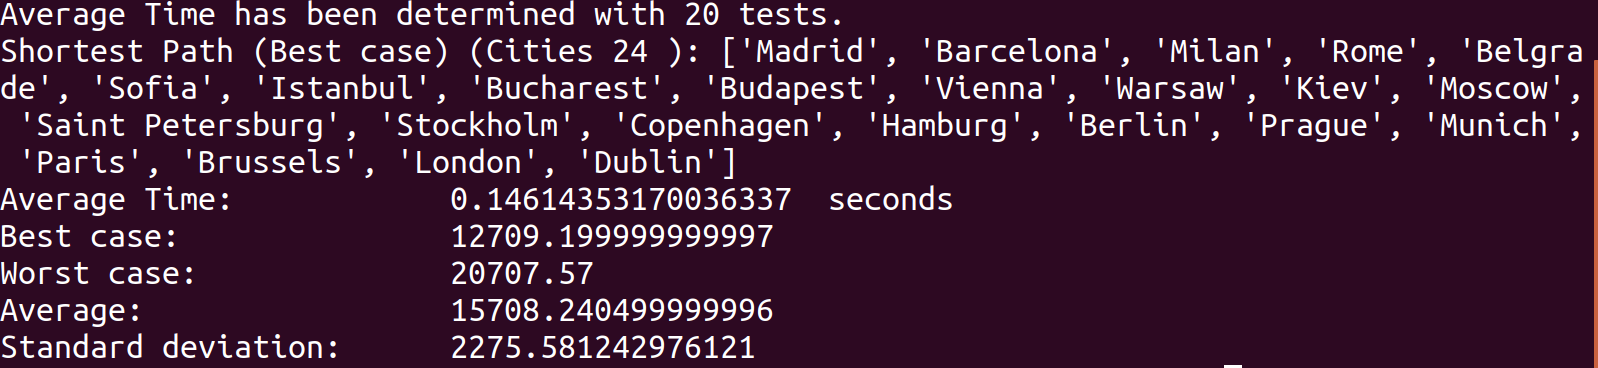
\includegraphics[width=1\linewidth]{pictures/hillClimbing/cities24}
		Hill Climbing Result, 24 Cities, 20 runs
	\end{center}
%%%%%%%%%%%%%%%%%%%%%%%%%%%%%%%%%%%%%%%%%%%%%%%%%%%%%%%%%%%%%%%%%%%%%%%%%%%%%%%	
% Genetic Algorithm
	\section{Genetic Algorithm}
%%%%%%%%%%%%%%%%%%%%%%%%%%%%%%%%%%%%%%%%%%%%%%%%%%%%%%%%%%%%%%%%%%%%%%%%%%%%%%%
% Genral
\subsection{General}
	\begin{tabular}{ l l } 
		Representation: 	& List of destinations (Adjacency Representation) \\
		Recombination: 		& Partially Mapped Crossover (PMX) \\
		Mutation: 			& Inversion Mutation (Because of the adjacency problem)	\\
		Parent Selection:	& Tournament Selection (Fitness-Proportionate-Selection)	\\
		Survivor Selection:	& Elitism, preserve the N best individuals. Other randomly(Exploration)\\ 
	\end{tabular}
%%%%%%%%%%%%%%%%%%%%%%%%%%%%%%%%%%%%%%%%%%%%%%%%%%%%%%%%%%%%%%%%%%%%%%%%%%%%%%%
% Code Overview	
	\subsection{Code overview}
	\begin{center}
		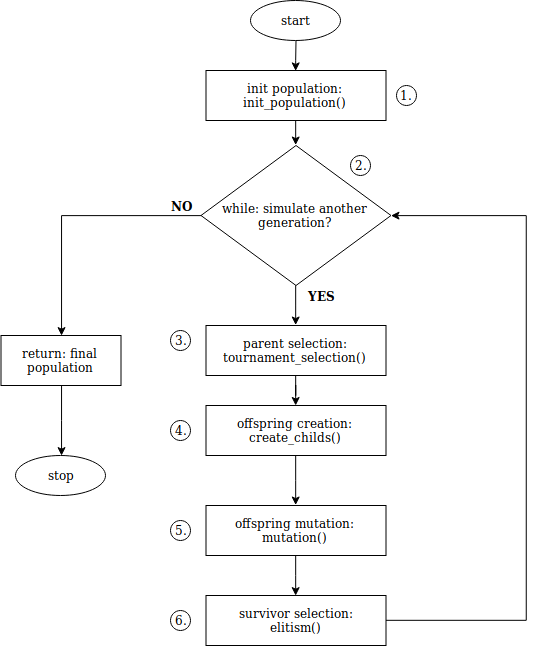
\includegraphics[width=0.9\linewidth]{pictures/geneticAlgorithm/genetic_algorithm}
		\\
		Graphical representation of the main procedure of \textit{genetic\_algorithm.py}
		\\
	\end{center}
	The graphic above show the fundamental procedure of the \textit{genetic\_algorithm} program. There are several steps in this program, i would like to explain in detail.\\
	\begin{enumerate}
	\item Initialization of the Population:	\\
	Firstly, a certain size of individuals will be created randomly to initialize the population.
	
		
	\item Loop: \\
	This loop provides a simulation of several generations.
	
	\item Parent Selection: \\
	This function selects a number of individuals that are able to create new children. The selection is made by a Tournament-Selection. There are two parameter that steers the selection. The first one is the \textit{number\_of\_tournament\_winners} that says how many parents should win the tournament. The second parameter is the \textit{tournament\_size} that determines the number of individuals that are compared to each other (This parameter steers the \textit{selection pressure}). The best individual will be selected. The tournament is created randomly.
	
	\item Offspring Creation: \\
	The tournament winners can now create new children. Each winner-parent can create children with any other winner-parent. To determine the combinations the function  \textit{combinations()} from  \textit{itertools} is used. Each combination will be executed with a certain \textit{crossover\_rate}. The crossover will be done by the pmx-function that you can find in the file \textit{PMX.py} (Because of the adjacency-based problem).
	
	\item Offspring Mutation: \\
	Each offspring will be modified with a certain \textit{permutation\_rate}. The inversion-mutation is used because it breaks only two links. That is an advantage for our kind of problem. 
	
	\item Survivor Selection: \\
	The survivor selection follows the \textit{elitism} principle. The \textit{N} best individuals will be selected for the next generation. The other \textit{populations\_size - N} individuals will be selected randomly, because for the reason of Exploration. Without this random selection, the algorithm converges very fast.
	\end{enumerate}	
	
%%%%%%%%%%%%%%%%%%%%%%%%%%%%%%%%%%%%%%%%%%%%%%%%%%%%%%%%%%%%%%%%%%%%%%%%%%%%%%%	
%Use the program	
	\subsection{Use the program}
	\subsubsection{Run the program}
	To run the program just execute the file: 
	\begin{center}
		\textit{python3 genetic\_algorithm.py}
	\end{center}
	\subsubsection{Change parameter}
	\begin{center}
		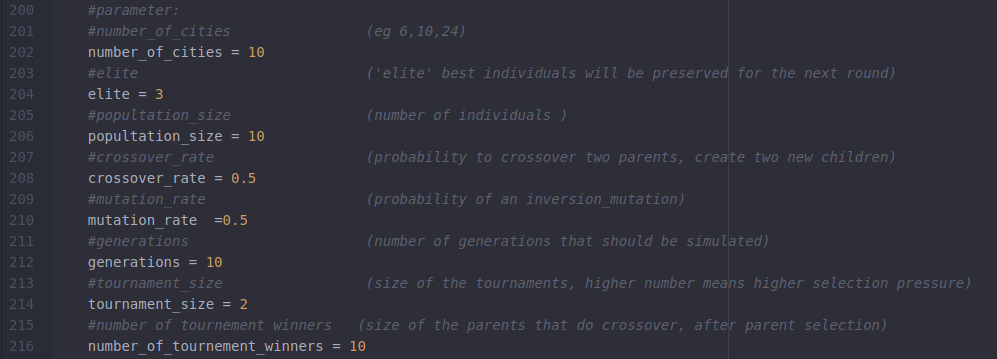
\includegraphics[width=1\linewidth]{pictures/geneticAlgorithm/parameter}
	\\
	Parameter that can be changed in the file \textit{genetic\_algorithm.py}.
	\\	
	\end{center}
	
	\subsection{Results of changing parameter}
	\subsubsection{Crossover Rate, Permutation Rate}
	\begin{center}
		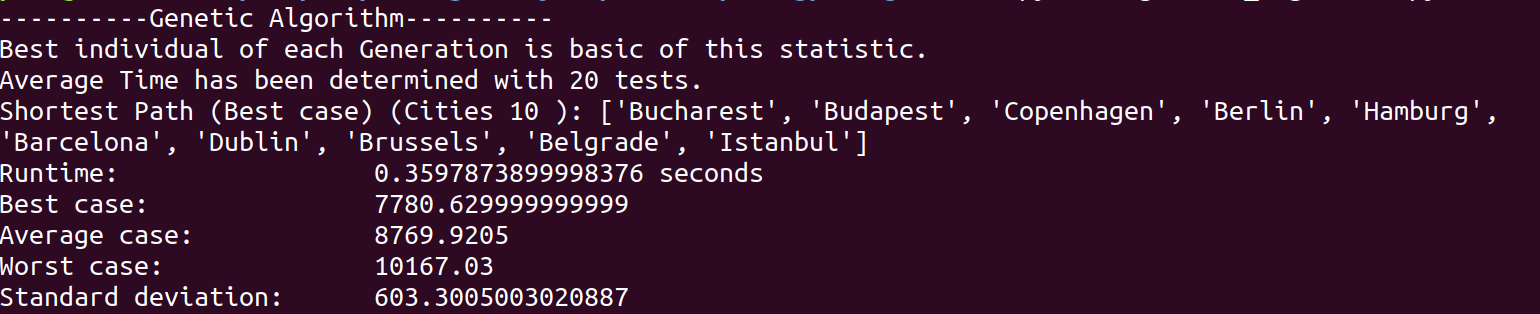
\includegraphics[width=1\linewidth]{pictures/geneticAlgorithm/rate0_1}
		\\
		Permutation Rate and Crossover Rate: 10\% (0.1)
		\\
	\end{center}
	\begin{center}
		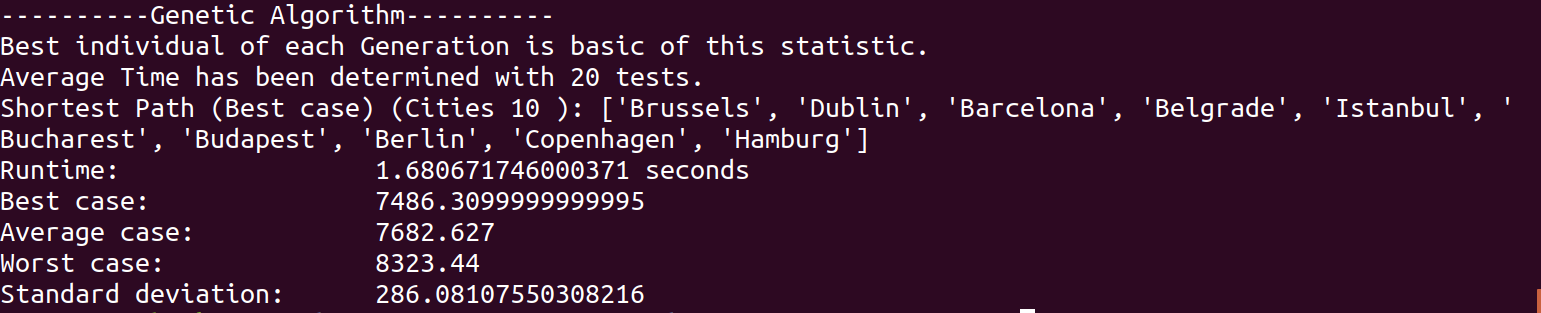
\includegraphics[width=1\linewidth]{pictures/geneticAlgorithm/rate0_9}
		\\
		Permutation Rate and Crossover Rate: 90\% (0.9)
		\\
	\end{center}
	More Mutations and Crossover means a better result but also more time to do this operations.
	
	\subsubsection{Number of Elite Survivor}
	\begin{center}
		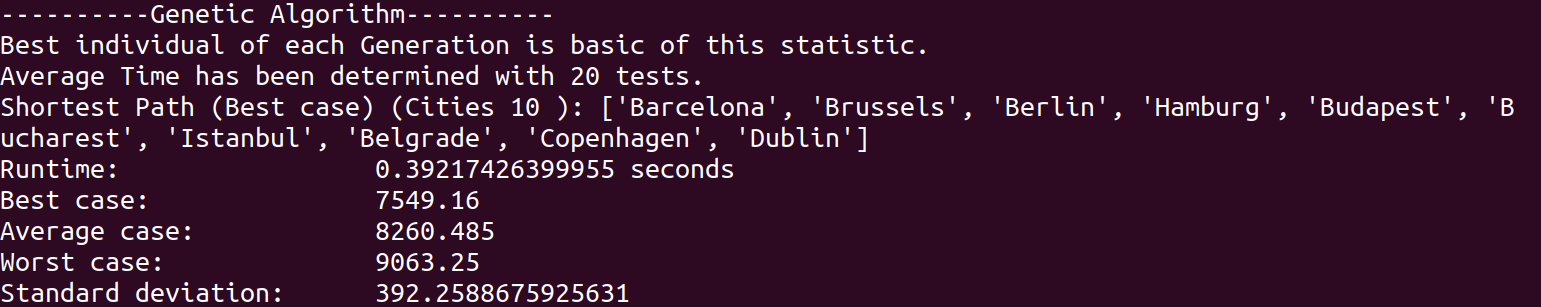
\includegraphics[width=1\linewidth]{pictures/geneticAlgorithm/10elite}
		\\
		10\% of the best children will be kept.
		\\
	\end{center}
	\begin{center}
		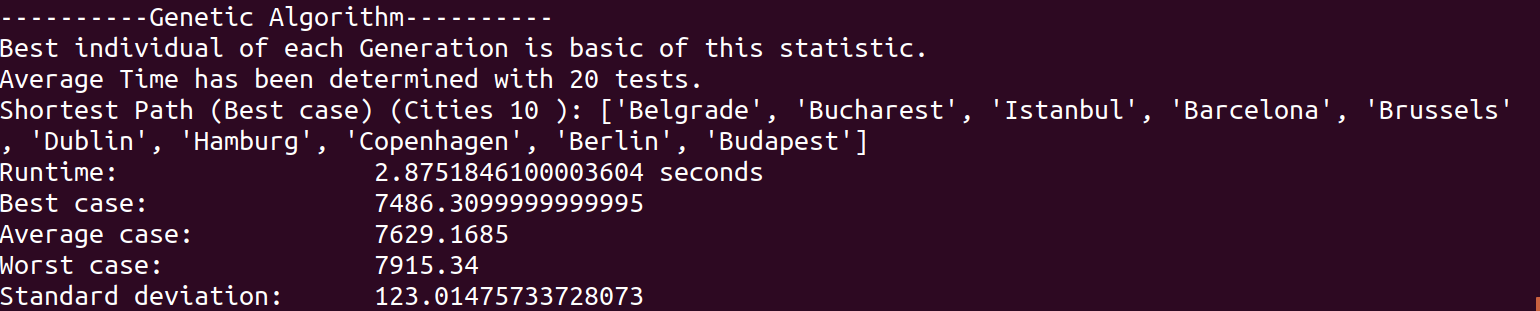
\includegraphics[width=1\linewidth]{pictures/geneticAlgorithm/90elite}
	\\
	90\% of the best children will be kept.
	\\	
	\end{center}
	The more better solutions are kept, the more better is the result. But that means also a much smaller deviation. That can easily result in local minimum because the solutions are very similar.
	
	\subsubsection{Number of Generations}
	\begin{center}
		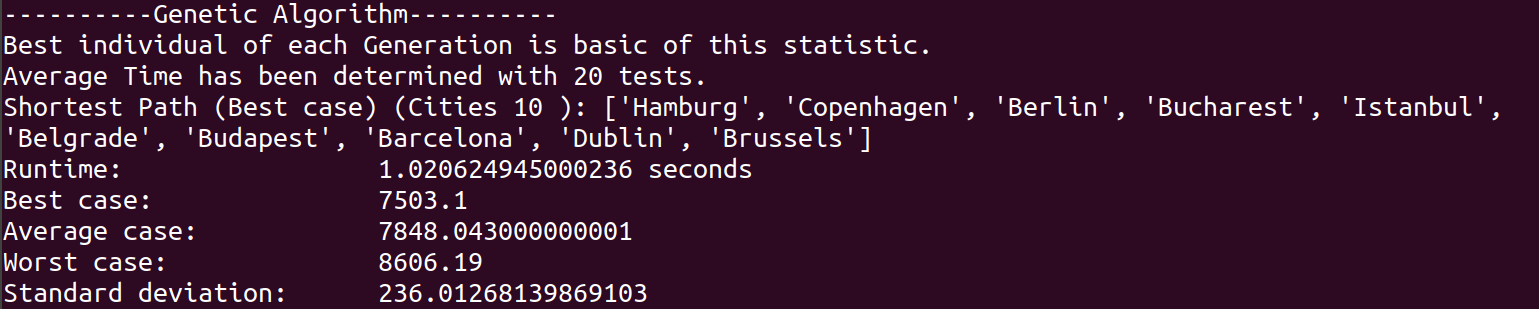
\includegraphics[width=1\linewidth]{pictures/geneticAlgorithm/10gen}
		\\
		10 Generations
		\\
	\end{center}
	\begin{center}
		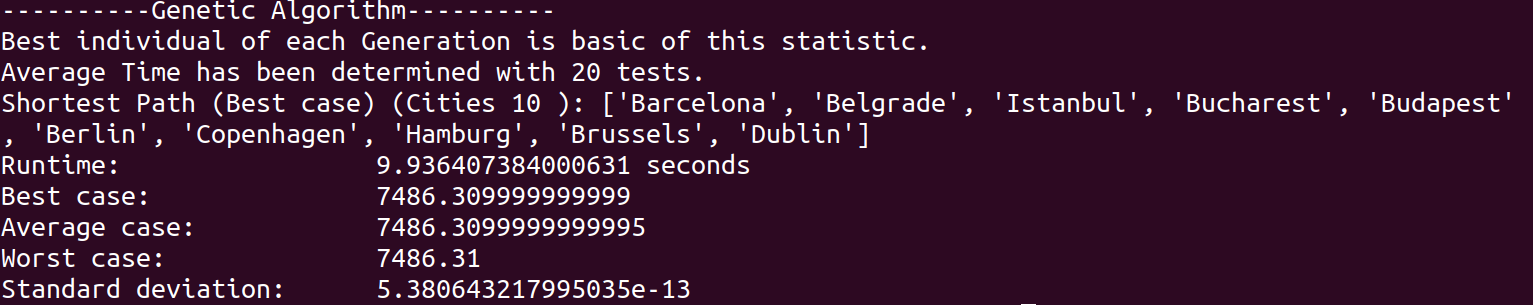
\includegraphics[width=1\linewidth]{pictures/geneticAlgorithm/100gen}
		\\
		100 Generations
		\\
	\end{center}
	The more generations there are, the better is the result of course. I think is the best way to improve the result. But it also takes much more time for the result.
	
	
	\subsubsection{Size of Population, 3 different sizes (Average across runs)}
	\begin{center}
		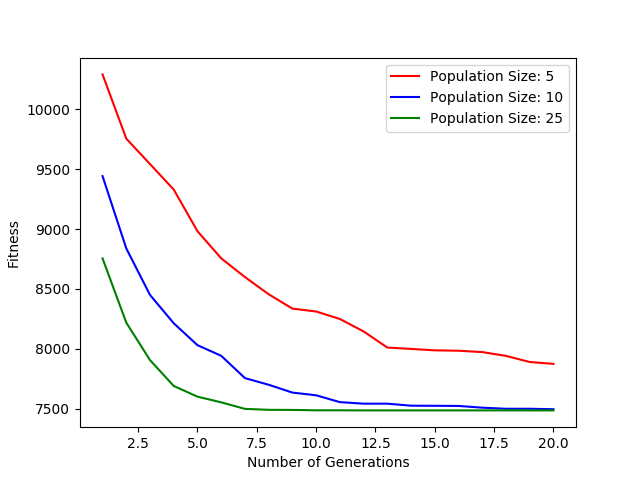
\includegraphics[width=1\linewidth]{pictures/geneticAlgorithm/genetic_all_in_one}
		\\
		20 runs, 3 different sizes of population, average of best individual
		\\
	\end{center}
	The bigger the population size is, the faster the algorithm converges. A reason for this is that a bigger population has from the beginning more better solution. That makes sense because the population is created randomly.\\
	As elitism is used, it is more likely that better solutions create new offspring. So that is why the biggest population (green line) has from the beginning very good individuals and converges very fast.
	
	\subsubsection{Tournament size}
	\begin{center}
		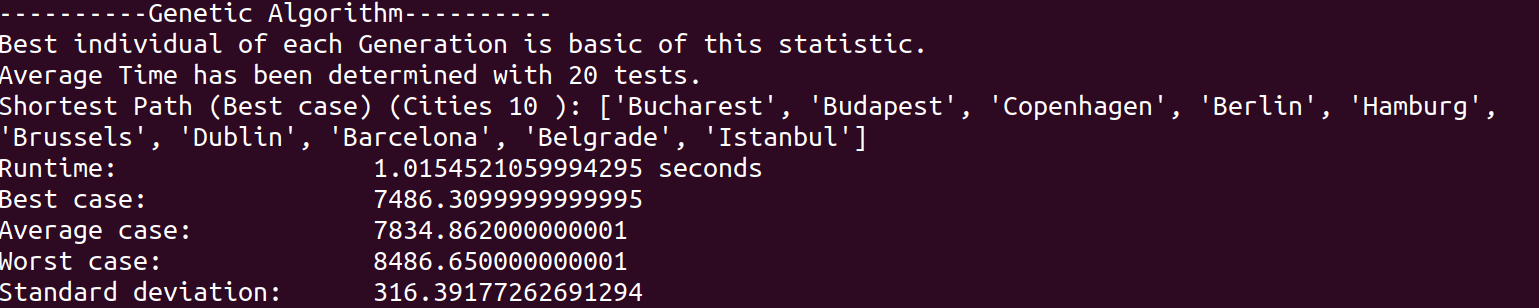
\includegraphics[width=1\linewidth]{pictures/geneticAlgorithm/2tourn}
		\\
		Tournament size of 2.
		\\
	\end{center}
	\begin{center}
		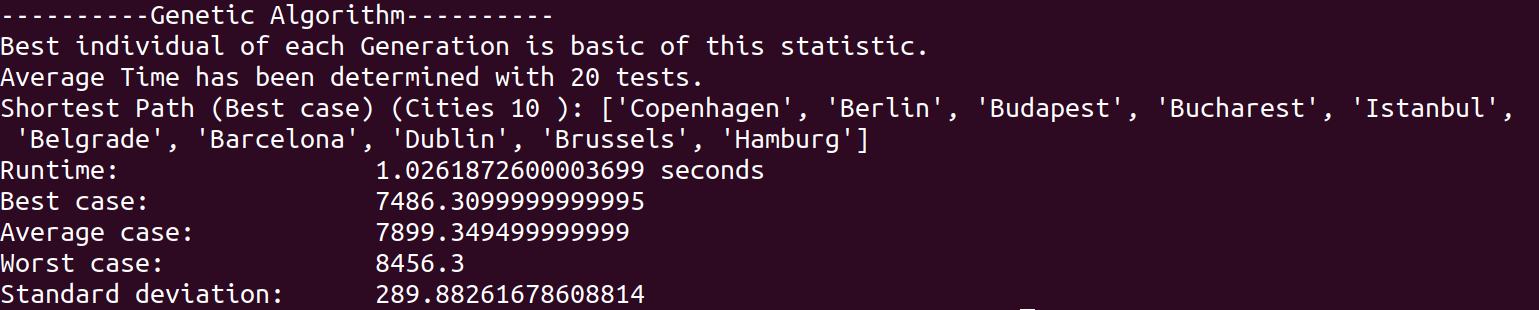
\includegraphics[width=1\linewidth]{pictures/geneticAlgorithm/8tourn}
			\\
		Tournament size of 8.
		\\
	\end{center}
	A higher tournament size means a better population quality (lower deviation). Because the selection pressure is higher.
	
	\subsubsection{Number of tournament winner}
	\begin{center}
		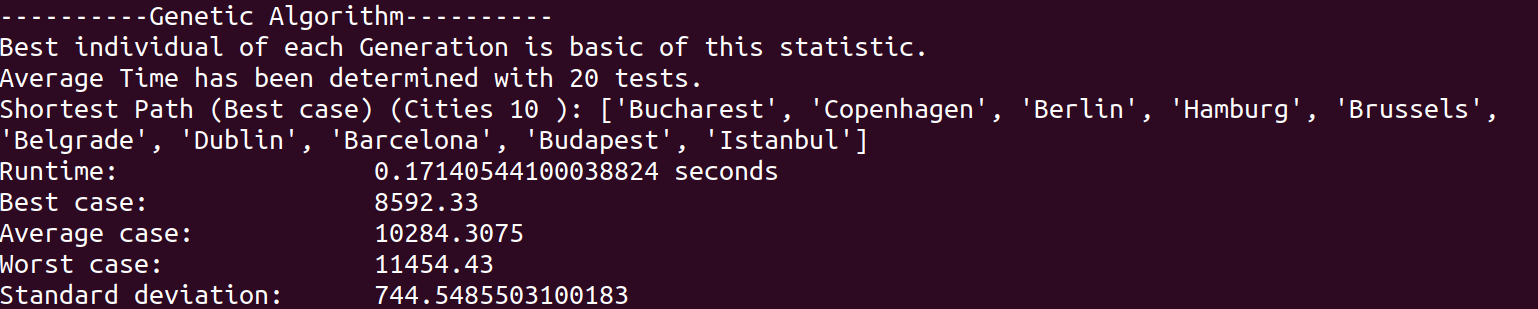
\includegraphics[width=1\linewidth]{pictures/geneticAlgorithm/tournwin10}
		\\
		10\% of the parents win the tournament. 
		\\
	\end{center}
	\begin{center}
		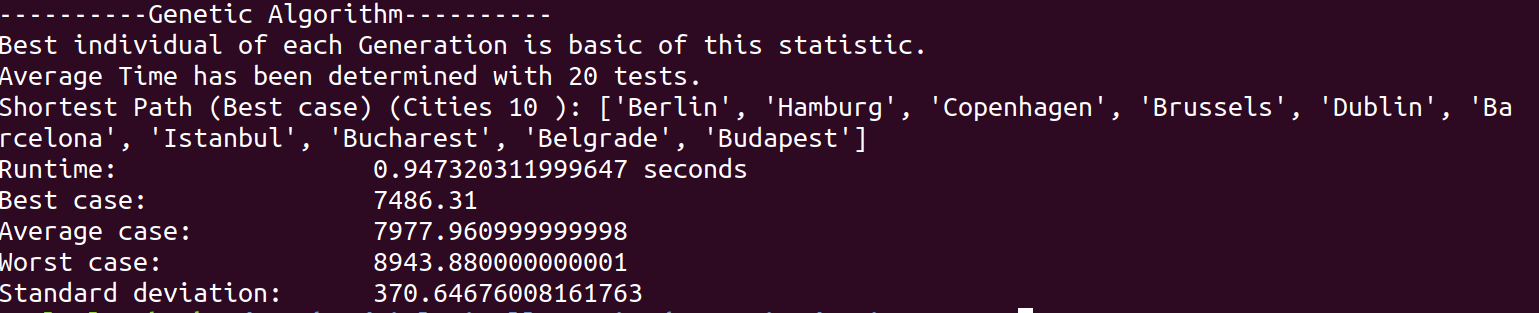
\includegraphics[width=1\linewidth]{pictures/geneticAlgorithm/tournwin90}
			\\
		90\% of the parents win the tournament. 
		\\
	\end{center}
	The more parents win the tournament, the more offspring will be created. That means also more diversity and a higher probability for a good solution.
	
	
	
%%%%%%%%%%%%%%%%%%%%%%%%%%%%%%%%%%%%%%%%%%%%%%%%%%%%%%%%%%%%%%%%%%%%%%%%%%%%%%%
%Questions		
	\subsection{Questions}
	\subsubsection{Result 6 Cities, 20 runs}
	\begin{center}
		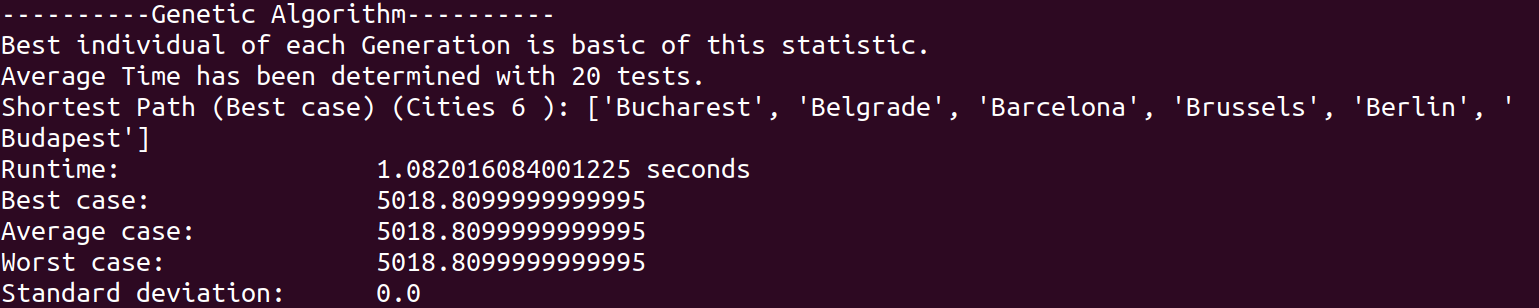
\includegraphics[width=1\linewidth]{pictures/geneticAlgorithm/cities6}
		\\
		20 Generations, 6 Cities
		\\
	\end{center}
	
	
	\subsubsection{Result 10 Cities, 20 runs}
	\begin{center}
		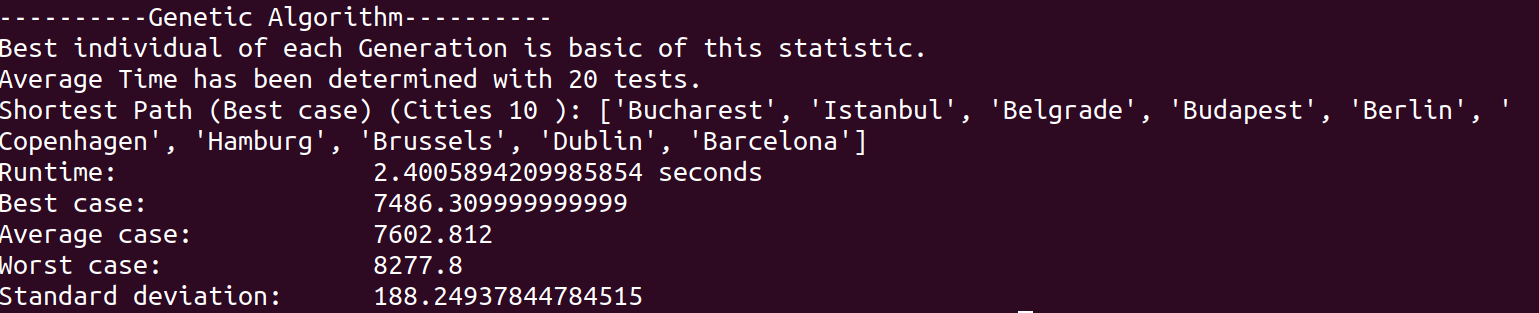
\includegraphics[width=1\linewidth]{pictures/geneticAlgorithm/cities10}
		\\
		20 generations, 10 Cities	
		\\
	\end{center}
	\begin{center}
		\begin{tabular}{ | c |c | c | c | c|}
			\hline
			Algorithm & Runs & Best solution & Runtime & Compared tours \\ \hline
			Exhaustive Search & 20 & 7486 & 84.4 s  & 3,628,800 \\ \hline
			Genetic Algorithm & 20 & 7486 & 2.4 s & 100* \\ 
			\hline
		\end{tabular}
	\end{center}
	100*: 10 Generations with population size of 10 \\
	We can see, that the GA finds also the best solution in a much shorter time.

	
	\subsubsection{Result 24 Cities, 20 runs}
	\begin{center}
		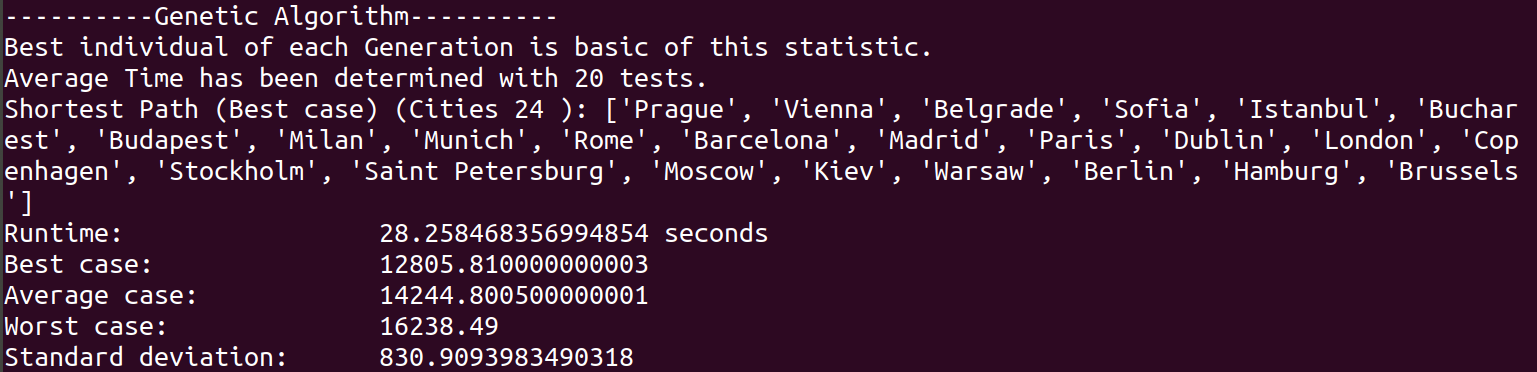
\includegraphics[width=1\linewidth]{pictures/geneticAlgorithm/cities24}
		\\
		100 generations, 24 Cities
		\\
	\end{center}
		\begin{center}
		\begin{tabular}{ | c |c | c | c | c|}
			\hline
			Algorithm & Runs & Best solution & Runtime & Compared tours \\ \hline
			Exhaustive Search & 20 & 7486 & -**  & $6.2\times10^{23}$ \\ \hline
			Genetic Algorithm & 20 & 12,805 & 28.3 s & 1000* \\ 
			\hline
		\end{tabular}
	\end{center}
	1000*: 100 Generations with population size of 10 \\
	-**: Not possible to compute
	
	
%%%%%%%%%%%%%%%%%%%%%%%%%%%%%%%%%%%%%%%%%%%%%%%%%%%%%%%%%%%%%%%%%%%%%%%%%%%%%%%		

\end{document}